\chapter{Dinamiche nelle Reti - Processi di Diffusione}

Uno dei quesiti principali fin ora posti è cercare di capire come le scelte dei singoli individui sono influenzate dal comportamento degli altri individui. Quando si fa questo tipo di analisi si può considerare la rete sottostante in due differenti livelli di risoluzione: un livello in cui guardiamo la rete dall'alto e osserviamo il comportamento di gruppi di individui, e un livello più dettagliato in cui si considera la struttura della rete come grafo e si cerca di analizzare/intuire come i singoli individui sono influenzati dal loro diretto vicinato.

In questa parte verrà analizzato il secondo punto di vista, assumendo che i singoli individui abbiano solo una visione locale della rete, e non globale, e di conseguenza che prendano decisioni in base a ciò che osservano (ovvero in base al comportamento dei loro vicini). Questo framework è abbastanza ragionevole, in quanto è ragionevole pensare che una persona venga influenzata e cambi comportamento in base al gruppo in cui appartengono, ricevendo così benefici. Per esempio è conveniente che una persona adotti una nuova lingua perché la grande maggioranza delle persone con cui a che fare parlano tale lingua, fregandosene di quale sia la lingua più parlata in assoluto al livello globale.

Questi ragionamenti sono alla base del concetto di \textbf{omofilia}. Per omofilia da una parte si intende la capacità che ha un individuo di creare relazioni con altri individui che più gli assomigliano (riferendoci per esempio alla chiusura triadica), e dall'altra parte è la tendenza a cercare di assomigliare a chi li circonda in modo tale da trarne vantaggi. Per esempio in un contesto sociale reale le persone tendono a creare rapporti con altre persone che hanno stessi gusti e/o opinioni, d'altro canto però spesso per ridurre la tensione sociale si tende a scendere a compromessi adattandosi a ciò che vogliono gli altri.

\section{Coordination Game - Modello Lineare}

Come ogni altro argomento, partiamo da degli esempi reali, e proviamo in seguito a formalizzare un modello che descriva al meglio l'esempio studiato.
Iniziamo con parlare del \textit{processo di diffusione delle innovazioni}. Esso è stato studiato in sociologia già a partire dalla metà del secolo scorso. Ryan e Gross, hanno osservato il processo di adozione di nuovi semi ibridi di mais da parte di un gruppo di agricoltori di Iowa. Sebbene la maggior parte degli agricoltori veniva a conoscenza dei nuovi semi tramite
le comunicazioni dei venditori, a parte un numero limitato di agricoltori, la maggior parte degli agricoltori iniziava a usare i nuovi semi solo dopo aver osservato che un certo numero di vicini / conoscenti / amici li stava utilizzando.

Lo scopo quindi è di modellare un processo di diffusione in una rete. Per fare ciò bisogna innanzitutto definire delle regole in base alle quali un nodo decide di cambiare. Definiamo quindi un modello di decisioni \textbf{individuali}, ovvero non c'è una coalizione di gruppi di nodi per prendere collettivamente la stessa decisione, ma ciascun nodo decide per se stesso. Le scelte dei nodi, infatti, sono guidate da \textbf{motivazioni di puro interesse personale}.

Assumiamo quindi che, nella rete si sia stabilizzato una certo stato $B$, e che, ad un certo istante, alcuni individui cambino il loro stato in $A$. La domanda che ci poniamo ora è: \textit{in quali casi un individuo decide di cambiare il proprio stato da $B$ a $A$?} (Inoltre, assumiamo che una volta passato da $B$ a $A$, non si può più tornare indietro).

Il modello che stiamo considerando si basa sul concetto di \textbf{Network Coordination Game}.

\begin{definizione}[Modello del Processo di Diffusione]
    Sia $G = (V, E, \{A, B\})$ la nostra rete, e consideriamo l'arco $(u, v) \in E$. A ciascun stato $A, B$, associamo un beneficio, rispettivamente $a, b$ (\autoref{tab:benefici})

    
    \begin{table}[h!]
        \centering
        \begin{tabular}{|c|c|c|}
        \hline
        \diagbox{$u$}{$v$} & A & B \\ \hline
        A & \rule{0pt}{14pt}$a,a$ & \rule{0pt}{14pt}$0,0$ \\ \hline
        B & \rule{0pt}{14pt}$0,0$ & \rule{0pt}{14pt}$b,b$ \\ \hline
        \end{tabular}
        \caption{Tabella dei benefici}
        \label{tab:benefici}
    \end{table}
    \begin{itemize}
        \item Se $u$ e $v$ adottano entrambi lo stato $A$, allora entrambi hanno un beneficio pari ad $a$;
        \item Se $u$ e $v$ adottano entrambi lo stato $B$, allora entrambi hanno un beneficio pari ad $b$;
        \item Altrimenti, nessuno dei due ha alcun beneficio.
    \end{itemize}
\end{definizione}

Ovviamente il nodo $v$ gioca una copia del coordination game su ognuno dei suoi archi incidenti, perciò il suo guadagno sarà la somma di tutti i guadagni su ogni arco.
Andiamo ora ad analizzare quando al nodo $v$ conviene adottare lo stato $A$ oppure no, sapendo che parte dallo stato $B$.

Definiamo con $n_A$ ed $n_B$ il numero dei suoi vicini rispettivamente negli stati $A$ e $B$. Intuitivamente viene da pensare che $v$ agisce nei seguenti modi:
\begin{itemize}
    \item Se $bn_B > an_A$ allora gli conviene rimanere in $B$.
    \item Se $an_A > bn_B$ allora gli conviene adottare $A$.
\end{itemize}

Assumiamo che nel caso di parità di guadagno venga comunque preferita l'innovazione $A$ anziché rimanere nello stato attuale. Perciò si adotta lo stato $A$ se $an_A \geq bn_B$.

Supponiamo che una porzione $p$ dei vicini di $v$ sia nello stato $A$, e che una frazione $1-p$ sia nello stato $B$
\begin{align*}
    p &= \frac{n_A}{| N(v) |}\\
    1-p &= \frac{n_B}{| N(v) |} = \frac{| N(v) | - n_A}{| N(v) |}
\end{align*}
Perciò possiamo dire che a $v$ conviene cambiare stato se
\begin{align*}
    n_A a &\geq n_B b\\
    (| N(v) | \cdot p) a &\geq (| N(v) | \cdot (1-p)) b\\
    p a &\geq (1-p)b\\
    p &\geq \frac{b}{a+b}
\end{align*}

\begin{definizione}[Soglia di Adozione]
Definiamo la soglia di adozione
\[
q = \frac{b}{a+b}
\]
la frazione minima dei vicini di $v$ che devono essere nello stato $A$ per rendere l'adozione di $A$ conveniente rispetto a $B$.
\end{definizione}

\begin{itemize}
    \item Se $a >> b$, allora $q$ è molto piccolo, quindi occorrono pochi vicini nello stato $A$ per indurre un nodo a cambiare stato (questo accade quando $A$ è migliore dello stato $B$).
    \item Se $a = b$, occorrono almeno la metà dei vicini nello stato $A$ per indurre un nodo a cambiare stato.
    \item Se $a << b$, allora $q$ è molto alto, quindi occorrono molti più vicini nello stato $A$ per indurre un nodo a cambiare stato (questo accade quando $A$ è peggiore dello stato $B$).
\end{itemize}

\section{Comportamento a Cascata}

Dobbiamo ora capire se esistono delle configurazioni di equilibrio, ovvero una configurazione del grafo nella quale non c'è più la transizione dallo stato $B$ allo stato $A$. Osserviamo che esistono 2 tipologie di configurazioni di equilibrio:
\begin{enumerate}
    \item Quando $A$ non è stato introdotto nella rete, cosicché tutti i nodi rimangono nello stato $B$.
    \item Quando, dopo che $A$ è stato introdotto nella rete, tutti i nodi sono passati nello stato $A$.
\end{enumerate}

Ovviamente la seconda configurazione è più interessante da studiare, in quanto bisogna capire quando termina il processo di diffusione, se lo stato $A$ riesce a raggiungere tutti i nodi, oppure, talvolta, la diffusione si blocca (e perché si blocca) ancor prima di aver raggiunto tutti i nodi, e porta la rete in configurazioni intermedie.

%\newpage

\subsection{Esempio 1}

Consideriamo il processo di diffusione dello stato $A$ nella rete in \autoref{fig:Diff_ex1}. Lo stato $A$ è stato forzato all'inizio sui nodi $v$ e $w$. Poniamo i guadagni $a = 3$ e $b = 2$, ottenendo come soglia di adozione $q = \frac{2}{5}$, ossia, almeno $q$ vicini di un nodo devono trovarsi nello stato $A$ affinché venga adottato dal nodo stesso. Nell'esempio in questione, i nodi $r$ e $t$ passeranno allo stato $A$, in quanto hanno entrambi $\frac{2}{3} > \frac{2}{5}$ vicino nello stato $A$. Successivamente, anche $s$ e $u$, ottenendo così una diffusione totale dello stato $A$ rispetto allo stato $B$

\begin{figure}[ht!]
    \centering
    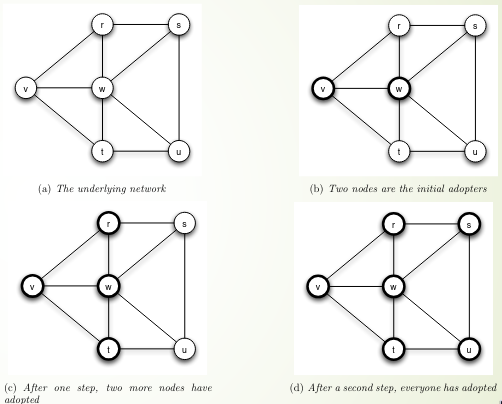
\includegraphics[width=0.5\linewidth]{images/Diff_ex1.png}
    \caption{Processo di diffusione in una rete}
    \label{fig:Diff_ex1}
\end{figure}

Se invece ponessimo come valori $a = 1$ e $b = 3$ , avremmo una soglia di adozione pari a $q = \frac{3}{4}$ , la quale non sarebbe sufficiente per la diffusione di $A$.

\subsection{Esempio 2}\label{sec:esempio2}

Consideriamo ora il processo di diffusione nella seguente rete (\autoref{fig:Diff_ex2}), e consideriamo due casistiche.

\begin{figure}[ht!]
    \centering
    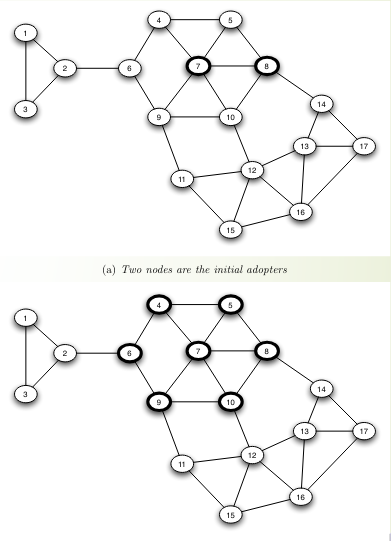
\includegraphics[width=0.25\linewidth]{images/Diff_ex2.png}
    \caption{Processo di diffusione in una rete}
    \label{fig:Diff_ex2}
\end{figure}

\begin{itemize}
    \item Se $a = 3$ e $b = 2$, allora $q = \frac{2}{5}$. In questo caso, (\autoref{fig:Diff_ex2}), lo stato $A$ è forzato sui nodi 7 e 8 e si diffonde solo sui nodi (4, 5, 6, 9, 10). Quindi $A$ non riesce a raggiungere i nodi fuori l'esagono.
    \item Se $a = 4$ e $b = 2$, allora $q = \frac{1}{3}$. In questo caso, dopo aver raggiunto tutti i nodi dell'esagono, $A$ è adottato anche da 2, 11 e 14, poi da 1, 3, 12, 13, 17 e infine da 15 e 16. In questo caso $A$, riesce a raggiungere tutti i nodi della rete.
\end{itemize}

Per riuscire ad ottenere una cascata completa, possiamo o aumentare il guadagno di $A$, oppure aumentare e/o cambiare i nodi iniziali nello stato $A$ (senza alterare la soglia d'adozione $q$ ). Per esempio consideriamo come insieme di nodi iniziali nello stato $A$ i nodi $\{2, 7, 8, 12\}$ (e ricordiamo che $q = \frac{2}{5}$ è rimasta invariata).

È facile osservare in questo caso che $A$ si propaga su tutta la rete.
Quindi, se non alteriamo $q$, viene da pensare che se il numero di nodi iniziali supera una certa soglia critica, allora avviene una cascata completa di $A$. In realtà l'avvenire di una cascata completa di $A$ non dipende solamente da quanti nodi iniziali sono forzati nello stato $A$, bensì anche dalla loro posizione. Per esempio se consideriamo altri 4 nodi iniziali $\{2, 7, 8, 14 \}$ non otterremo una cascata completa, nonostante ci siano lo stesso 4 nodi iniziali che adottano $A$.

\section{Cascate e Cluster}

\begin{definizione}[Insieme di Iniziatori]
    Definiamo l'insieme di nodi iniziatori $V_0$, l'insieme di nodi di partenza su cui viene forzato lo stato $A$. Indichiamo inoltre con $V_i$, l'insieme di nodi che adottano lo stato $A$ al passo $i$ del processo di diffusione.
\end{definizione}

\begin{definizione}[Cascata Completa]
    Definiamo il concetto di \textbf{cascata completa}, se ad un certo passo $t$, tutti i nodi hanno adottato $A$, ossia
    \[
    \text{se esiste } t \geq 0 \text{ tale che } \bigcup_{0 \leq i \leq t}V_i = V 
    \]

    Possiamo dire che la diffusione di $A$ si ferma quando 
    \[
    \bigcup_{i = 0}^{t} V_i = \bigcup_{i = 0}^{t+1} V_i
    \]
\end{definizione}

\begin{definizione}[Cluster di Densità $p$]
    Un \textbf{cluster di densità} $p$ è un sottoinsieme di nodi $V' \subseteq V$ tale che la frazione di vicini che ogni suo nodo ha in $V'$ è almeno $p$:
    \[
    \forall\ u \in V'\ \left[\frac{|N(u) \cap V'|}{|N(u)|} \geq p\right]
    \]
\end{definizione}

\begin{osservazione}
    Osservare anche che se $V',V''$ sono due cluster di densità $p$, allora anche $V' \cup V''$ è un cluster di densità $p$.
\end{osservazione}

\begin{proof}
Supponiamo $V'\cap V''=\varnothing$ e sia $u\in V'\cup V''$.

\textbf{Caso 1:} $u\in V'$. Allora, essendo $V'$ un cluster di densità $p$,
\[
\frac{|N(u)\cap V'|}{|N(u)|}\ge p.
\]
Poiché $V'\subseteq V'\cup V''$, si ha $N(u)\cap V'\subseteq N(u)\cap (V'\cup V'')$, dunque
\[
\frac{|N(u)\cap (V'\cup V'')|}{|N(u)|}\ge\frac{|N(u)\cap V'|}{|N(u)|}\ge p.
\]

\textbf{Caso 2:} $u\in V''$. Il ragionamento è identico scambiando i ruoli di $V'$ e $V''$.

Inoltre, poiché $V'\cap V''=\varnothing$, per ogni $u$ vale la relazione additiva
\[
|N(u)\cap (V'\cup V'')|=|N(u)\cap V'|+|N(u)\cap V''|,
\]
che mostra esplicitamente come i contributi provengano da insiemi disgiunti. Comunque, dai due casi precedenti segue che ogni nodo di $V'\cup V''$ ha almeno una frazione $p$ dei vicini nell'unione, quindi $V'\cup V''$ è un cluster di densità $p$.
\end{proof}

\begin{teorema}
    Sia $G = (V, E)$ un grafo e siano $V_0 \subseteq V$ l'insieme di nodi iniziatori e $q$ la soglia di adozione dello stato $A$.
    \[
        V_0 \text{ non genera una cascata completa}
        \quad\Longleftrightarrow\quad
        G \setminus V_0 \text{ contiene un cluster di densità } > 1-q .
    \]
\end{teorema}
\begin{proof}
    \mbox{}\\
    \textbf{($\implies$)}\; Supponiamo che $V_0$ non generi una cascata completa. In questo caso, esistono dei nodi che non adottano $A$. Quindi, sia $t$ il passo tale che $V_t \neq \emptyset$ e  $V_{t+1} = \emptyset$ (ossia $t + 1$ è il primo passo in cui $A$ non si diffonde più). Poniamo
    \[
    V_A = \bigcup_{0 \leq i \leq t} V_i
    \]
    l'insieme che contiene tutti e soli i nodi che adottano $A$. Poiché esistono nodi che non adottano $A$, allora $V \setminus V_A \neq \emptyset$. Poiché i nodi in $V \setminus V_A$ non adottano $A$, allora, \[
    \forall\ v \in V \setminus A\ \left[\frac{|N(v) \cap V_A|}{|N(v)|} < q\right]
    \]
    Quindi, poiché 
    \[
    \frac{|N(v) \cap V_A|}{|N(v)|} + \frac{|N(v) \cap (V \setminus V_A)|}{|N(v)|} = 1, \text{ allora } \frac{|N(v) \cap (V \setminus V_A)|}{|N(v)|} > 1-q
    \]
    In conclusione, $V \setminus V_A$ è un cluster di densità maggiore di $1 - q$ e $V \setminus V_A$ è contenuto in $G \setminus V_0$.
    \medskip

    \textbf{($\impliedby$)}\; Supponiamo ora che in $G \setminus V_0$ esista un cluster di densità maggiore di $1-q$. Ovvero, esiste $C \subseteq V \setminus V_0$ tale che, per ogni $v \in C$, $\frac{|N(v) \cap C|}{|N(v)|} > 1-q$.

    Supponiamo ora per assurdo che si generi una cascata completa: allora i nodi in $C$, prima o poi, adotteranno $A$. Sia $t$ il primo passo tale che $V_t \cap C \neq \emptyset$ (esistono nodi in $C$ che al passo $t$ hanno adottano $A$) ossia, per $i < t$, $V_i \cap C = \emptyset$ e di conseguenza esiste $u \in V_t \cap C$.

    Poniamo ora
    \[
    V' = \bigcup_{0 \leq i \leq t - 1} V_i
    \]
    l'insieme dei nodi che hanno adottato $A$ fino al passo $t - 1$, quindi $V'$ non contiene nessun nodo di $C$.
    Allora,
    \begin{itemize}
        \item Poiché $C$ è un cluster di densità $> 1 - q$ e $u \in C$, allora $\frac{|N(u) \cap C|}{|N(u)|} > 1-q$.
        \item Inoltre, poiché $u \in V_t$, allora $\frac{|N(u) \cap C|}{|N(u)|} \geq q$
    \end{itemize}
    Quindi, poiché $V' \cap C \neq \emptyset$, allora
    \[
    1  \textcolor{red}{ = } \frac{|N(u)|}{|N(u)|} \geq \frac{|N(u) \cap (C \cup V')|}{|N(u)|} = \frac{|N(u) \cap C|}{|N(u)|} + \frac{|N(u)| \cap V'|}{|N(u)|}  \textcolor{red}{ > } q + 1 - q = 1
    \]
    Trovando quindi un \textbf{\textcolor{red}{ASSURDO}}.
\end{proof}

Ciò che ci dice il precedente teorema è sostanzialmente che la presenza di cluster (con una certa densità) comporta un ostacolo alla diffusione di una innovazione $A$.

Ricordiamo dalle lezioni precedenti che generalmente i legami che collegano due comunità (o cluster) sono dei \textbf{legami deboli} (\textbf{weak ties}).
Infatti la forza dei \textbf{weak ties} è basata sull'idea che le connessioni sociali deboli (per esempio con persone che vediamo di rado) spesso formano \textbf{bridge edges} in una rete sociale.
Pertanto forniscono accesso a fonti di informazioni (per esempio nuove opportunità di lavoro) che risiedono in parti della rete a cui altrimenti non avremmo accesso.

Osserviamo inoltre che c'è una sostanziale differenza tra venire a conoscenza di una nuova idea e il decidere di adottarla.
Infatti considerando ancora l'esempio 2 (\autoref{sec:esempio2}), possiamo osservare che i nodi 4 e 9 vengono subito a conoscenza dell'innovazione $A$ in quanto entrambi sono vicini di un nodo iniziatore, però attendono più tempo prima di adottarlo.
Anche in un contesto sociale reale, sebbene una barzelletta o un video divertente online avanzano con una velocità notevole, la mobilitazione politica si muove più lentamente, avendo bisogno di prendere slancio all'interno di comunità.

La soglia di adozione $q$ offre una possibile spiegazione:
i movimenti sociali tendono ad essere imprese intrinsecamente rischiose, e quindi gli individui tendono a necessitare di soglie più elevate per la partecipazione.

Perciò possiamo concludere che mentre i \textit{weak-ties} che collegano due comunità differenti sono utilissimi alla diffusione di informazioni, allo stesso tempo sono un punto di debolezza (e quindi di ostacolo) per la diffusione di un'innovazione.

\newpage
\section{The Cascade Capacity on Infinite Network with bounded Degree}

In questa sezione analizzeremo in maniera più formale, tramite l'aiuto di alcuni esempi, se esiste e qual è la \textbf{threshold} (per una soglia di adozione) che scatena una cascata completa, anche con un insieme "piccolo" di nodi \textbf{iniziatori}.

Più in particolare analizzeremo il caso di reti con \textbf{infiniti nodi}, ma ognuno con \textbf{grado finito}. In questa maniera il concetto di \textit{insieme piccolo di iniziatori} è definito da qualsiasi \textbf{insieme finito}.


\begin{tcolorbox}[colback=white,colframe=black,title=Problema]
Dato un grafo regolare infinito \(G = (V, E)\), in cui ogni nodo possiede grado finito, si definisce la
\emph{soglia di adozione massima} \(q_{\mathrm{MAX}}\) come il valore più alto di \(q \in [0,1]\) per il quale
\emph{esiste} un insieme iniziale finito \(V_0 \subset V\) tale da innescare una cascata completa
nell'intero grafo secondo la dinamica di adozione basata sulla soglia.
\end{tcolorbox}

Il valore \(q_{\mathrm{MAX}}\) prende il nome di \textbf{capacità di cascata di} $G$.

\subsection{Esempio 1 - Catena Infinita}

Consideriamo una catena infinita di nodi, dove ogni nodo $i$ ha grado esattamente due ed incidente ai due archi $(i-1, i),\ (i, i+1)$.
Seppur tale insieme di nodi è equivalente all'insieme $\mathbb{Z}$, sappiamo che esiste una biezione con $\mathbb{N}$.

\begin{figure}[h!]
    \centering

    \begin{subfigure}{0.8\linewidth}
        \centering
        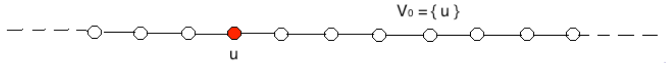
\includegraphics[width=\linewidth]{images/catena_infA.png}
        \caption{Primo caso: $V_0 = \{u\}$}
        \label{fig:catena_infinitaA}
    \end{subfigure}

    \vspace{0.5cm}

    \begin{subfigure}{0.8\linewidth}
        \centering
        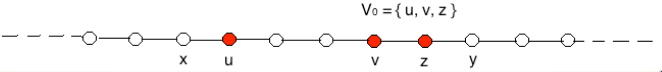
\includegraphics[width=\linewidth]{images/catena_infinitaB.png}
        \caption{Secondo caso: $V_0 = \{u, v, z\}$}
        \label{fig:catena_infinitaB}
    \end{subfigure}

    \caption{Grafo a catena infinita}
    \label{fig:catena_infinita}
\end{figure}


\begin{itemize}
    \item Se $|V_0| = 1$, ossia $V_0 = \{u\}$, allora occorre $q = \frac{1}{2}$ per generare una cascata completa, come mostrato in \autoref{fig:catena_infinitaA}.
    \item Se $|V_0| > 1$, ad esempio $V_0 = \{u, v, z\}$, è possibile generare una cascata con $q < \frac{1}{2}$? La risposta è \textbf{NO}, perché i nodi "al confine" con $V_0$, i nodi $x, y$ in \autoref{fig:catena_infinitaB}, hanno comunque bisogno di $q = \frac{1}{2}$ per passare ad $A$.
\end{itemize}

Quindi possiamo concludere che in una catena infinita, $q_{\mathrm{MAX}} = \frac{1}{2}$.

\newpage
\subsection{Esempio 2 - Grafo a Griglia Infinita}

Consideriamo ora una \textbf{griglia} infinita $\mathbb{Z} \times \mathbb{Z}$, dove ogni nodo è collegato coi nodi nelle rispettive posizione "UP", "DOWN", "LEFT", "RIGHT", "NE", "NW", "SE" e "SW".

\begin{figure}[ht!]
    \centering

    % Riga superiore
    \begin{subfigure}{0.23\linewidth}
        \centering
        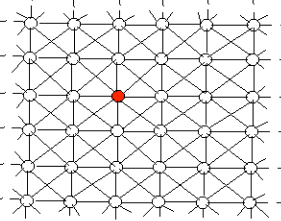
\includegraphics[width=\linewidth]{images/griglia.png}
        \caption{$|V_0| = 1$}
        \label{fig:griglia1}
    \end{subfigure}
    \hspace{0.1cm}
    \begin{subfigure}{0.23\linewidth}
        \centering
        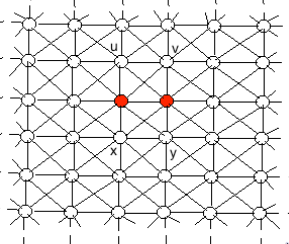
\includegraphics[width=\linewidth]{images/griglia2.png}
        \caption{$|V_0| = 2$}
        \label{fig:griglia2}
    \end{subfigure}

    % Riduzione drastica dello spazio verticale
    \vspace{0.2cm}

    % Riga inferiore
    \begin{subfigure}{0.23\linewidth}
        \centering
        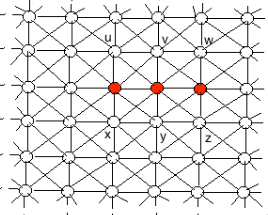
\includegraphics[width=\linewidth]{images/griglia3.png}
        \caption{$|V_0| = 3$}
        \label{fig:griglia3}
    \end{subfigure}
    \hspace{0.1cm}
    \begin{subfigure}{0.23\linewidth}
        \centering
        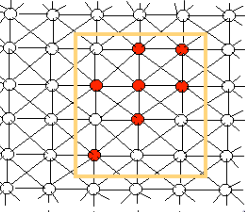
\includegraphics[width=\linewidth]{images/griglia4.png}
        \caption{$|V_0| > 3$}
        \label{fig:griglia4}
    \end{subfigure}

    \caption{Configurazioni di $V_0$ e soglie corrispondenti nella griglia.}
    \label{fig:griglia_totale}
\end{figure}


\begin{itemize}
    \item Se $|V_0| = 1$, allora occorre $q = \frac{1}{8}$ per generare una cascata completa.
    \item Se $|V_0| = 2$, allora $V_0$ contiene 2 nodi adiacenti e occorre $q = \frac{1}{4}$ per generare una cascata completa.
    \item Se $|V_0| = 3$, allora occorre $q = \frac{3}{8}$ per generare una cascata completa.
    \item Aumentando ulteriormente $|V_0|$, non si innalza più la soglia di adozione: per superare il rettangolo iniziale serve comunque $\frac{3}{8}$.
\end{itemize}

Allora, in una griglia infinita, $q_{\mathrm{MAX}} = \frac{3}{8}$.

\subsection{Soglia di Adozione Massima}

Dagli esempi precedenti è facile notare che la soglia di adozione massima nella griglia infinita è minore di quella della catena infinita, per via di una struttura più ricca è densa.
Comunque, in entrambi i casi, non si può mai avere una soglia di adozione maggiore di $\frac{1}{2}$

Quindi viene da pensare che, almeno in questi due modelli, l'innovazione $A$ deve essere appetibile almeno quanto lo stato dominante $B$.
In effetti questo è un ragionamento abbastanza ragionevole anche applicato in un contesto reale.

Sorge però la domanda:
\textit{Esiste una conformazione di una rete infinita in cui si può ottenere una capacita di cascata maggiore di $\frac{1}{2}$?}
\textit{Ovvero, è possibile fare in modo che si adotti $A$, nonostante $B$ sia più conveniente?}
Per fortuna la risposta è \textbf{NO}, e questo verrà dimostrato nel seguente teorema.

\begin{teorema}
    Per ogni grafo infinito $G=(V,E)$ i cui nodi hanno grado finito, la capacità di cascata di $G$ è al più $q_G \leq \frac{1}{2}$.
\end{teorema}

\begin{proof}
    Supponiamo per assurdo che esista un insieme finito di iniziatori $V_0$ che, con soglia di adozione $q > \frac{1}{2}$, generi una cascata completa.

    Indichiamo con $V_t$ l'insieme dei nodi che adottano $A$ al passo $t$. Sia, per ogni $t \geq 0$,
    \[
    S_t = \bigcup_{0 \leq i \leq t} Vi
    \]
    l'insieme dei nodi che, al passo $t$, sono nello stato $A$. 
    
    Definiamo l'\textbf{interfaccia $I_t$ al passo $t$} come l'insieme degli archi che, al passo $t$, hanno un estremo in $S_t$ e l'altro estremo in $V \setminus S_t$:
    \[
    I_t = \{(u, v) \in E: u \in S_t \land v \in V \setminus S_t\}
    \]
    In altre parole, $I_t$ è l'insieme di archi del \textbf{taglio} $(S_t, V \setminus S_t)$.

    Dato che $V_0$ genera una \textit{cascata completa} di $A$ con soglia di adozione $q > 0.5$, si può dimostrare che per ogni $t \geq 0$, allora è vero che 
    \[
    |I_t| > |I_{t+1}| \text{ oppure } I_t \equiv I_{t+1}
    \]

    Dato che il grado massimo di $G$ è \textbf{limitato}, allora $|I_0|$ sarà una quantità finita $k > 0$.
    Inoltre, è facile convincersi che il processo termina quando abbiamo che $I_t \equiv I_{t+1}$.
    
    Però visto che $V_0$ genera un processo \textbf{infinito} di cascata di $A$, allora per ogni $t \geq 0$, non deve mai accadere che $I_t \equiv I_{t+1}$, ovvero accade sempre che $|I_t| > |I_{t+1}|$.
    Ma ciò è assurdo, perché per via della dimensione finita di $I_0$, può accadere \textbf{al più} $k$ volte consecutive che il processo procedi.
    
    Perciò deve esistere necessariamente un tempo $\tau \geq k$, tale che $I_\tau \equiv I_{\tau + 1}$ (\textbf{\textcolor{red}{ASSURDO}}).

    Per farlo, basta dimostrare la \textbf{mutua esclusione} degli eventi, ovvero che se $I_t \not\equiv I_{t+1}$ allora necessariamente $|I_t| > |I_{t+1}|$\footnote{È stata applicata questa regola  $\lnot b \implies a \equiv a \lor b$ dove $a = |I_t| > |I_{t+1}|$ e $b = I_t \equiv I_{t+1}$.}.

    Quindi, se $I_t \not\equiv I_{t+1}$, allora esiste un nodo $v$ che adotta $A$ al passo $t + 1$, ossia $V_{t+1} \neq \emptyset$. Affinché ciò sia vero ($v \in V_{t+1}$), è necessario che $v$ abbia \textit{almeno} un vicino $u \in N(v)$ che è anche nello stato $A$, ovvero $u \in N(v) \cap S_t$. Più in generale, per ogni nodo $v \in V_{t+1}$ esiste almeno un arco del tipo $(u,v) \in I_t$, inoltre tale arco non apparterrà a $I_{t+1}$.
    Viceversa, tutti gli archi che apparterranno a $I_{t+1}$ certamente non erano in $I_t$.

    Quindi, per ogni $v \in V_{t+1}$,
    \begin{itemize}
        \item Gli archi incidenti su $v$ il cui altro estremo è in $S_t$ sono in $I_t$ ma non in $I_ {t+1}$ (come $(u,v)$ in \autoref{fig:PDdimostrazione}).
        \item Gli archi incidenti su $v$ il cui altro estremo è in $S_{t+1}$ sono in $I_{t+1}$ ma non in $I_t$ (come $(v, z)$ in \autoref{fig:PDdimostrazione}).
    \end{itemize}

    \begin{figure}[ht!]
        \centering
        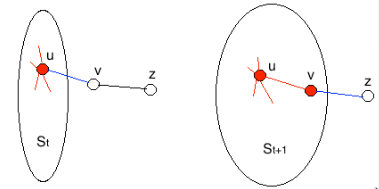
\includegraphics[width=0.5\linewidth]{images/PDdimostrazione.png}
        \caption{Gli archi di interfaccia sono disegnati blu}
        \label{fig:PDdimostrazione}
    \end{figure}

    Chiarito ciò, abbiamo che
    \[
    I_{t + 1} \equiv I_t \setminus \left[\bigcup_{v \in V_{t+1}} \lbrace (u,v) \in E : u \in S_t \right] \bigcup \left[\bigcup_{v \in V_{t+1}} \lbrace (z,v) \in E : z \in V \setminus S_{t+1} \right]
    \]

    È anche facile verificare che $\forall v,w \in V_{t+1},\ v \neq w$
    \begin{equation*}
        \begin{split}
        \{(u,v) \in E : u \in S_t \} &\cap \{ (u,w) \in E : u \in S_t \} = \emptyset\\
        &\land\\
        \{ (v,z) \in E : z \in V \setminus S_{t+1} \} &\cap \{ (w,z) \in E : z \in V \setminus S_{t+1} \} = \emptyset
        \end{split}
    \end{equation*}

    Per comprendere meglio ciò, visualizzare la \autoref{fig:PDdimostrazione2}

    \begin{figure}[ht!]
        \centering
        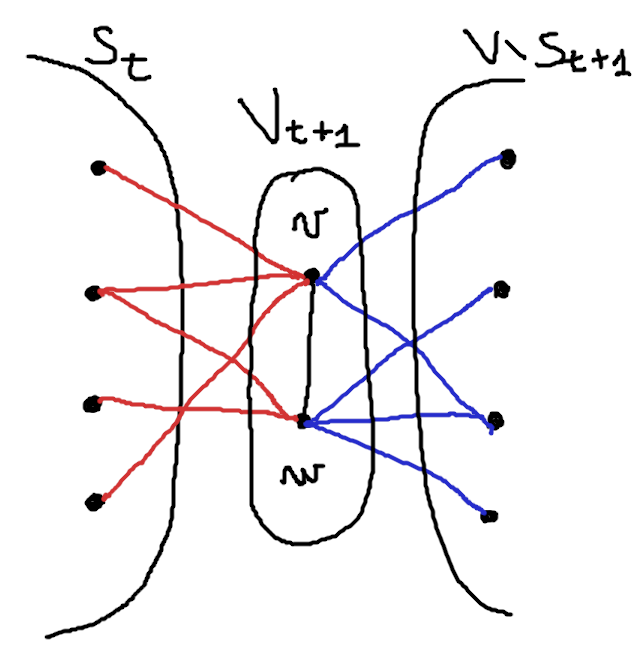
\includegraphics[width=0.3\linewidth]{images/PDdimostrazione2.png}
        \caption{Esempio}
        \label{fig:PDdimostrazione2}
    \end{figure}

    Tutto ciò implica che 
    \[
    |I_{t+1}| = |I_t| - \sum_{v \in V_{t+1}} |\{ (u,v) \in E : u \in S_t \}| + \sum_{v \in V_{t+1}} |\{ (v,z) \in E : z \in V \setminus S_{t+1} \}|
    \]

    Osserviamo ora, che,
    \[
    |\{ (u,v) \in E : u \in S_t \}| = |N(v) \cap S_t|
    \]
    e che
    \[
    |\{ (v,z) \in E : z \in V \setminus S_{t+1} \}| = |N(v) \setminus S_{t+1}|
    \]
    Infatti, per ogni \(v \in V_{t+1}\) vale che
    \[
    (u, v) \in I_t \iff u \in N(v) \cap S_t
    \]
    e analogamente
    \[
    (u,v) \in I_{t + 1} \iff u \in N(v) \setminus S_t
    \]
    Quindi, otteniamo
    \[
    |I_{t+1}| = |I_t| - \sum_{v \in V_{t+1}} |N(v) \cap S_t| + \sum_{v \in V_{t+1}} |N(v) \setminus S_{t+1}|
    \]

    Osserviamo adesso che, dato che un $v \in V_{t+1}$ ha adottato il nuovo stato $A$, e dato che la soglia di adozione è $q > \frac{1}{2}$, allora più della metà dei suoi vicini era in $S_t$, ovvero 
    \[
    \frac{| N(v) \cap S_t |}{| N(v) |} \geq q > \frac{1}{2}
    \]
    Oppure, visto in altri termini 
    \[
    | N(v) \cap S_t | > | N(v) \setminus S_t | \underbrace{>}_{\text{perché }S_t \subset S_{t+1}} | N(v) \setminus S_{t+1} |
    \]
    Allora, 
    \begin{align*}
        |I_{t+1}| &= |I_t| - \sum_{v \in V_{t+1}} |N(v) \cap S_t| + \sum_{v \in V_{t+1}} |N(v) \setminus S_{t+1}| \\
        &= |I_t| -  \sum_{v \in V_{t+1}} |N(v) \cap S_t| + |N(v) \setminus S_{t+1}| \\
        &\leq |I_t| - \sum_{v \in V_{t+1}} |N(v) \cap S_t| - |N(u) \setminus S_t|\\
        &= | I_t | - \sum_{v \in V_{t+1}} 1 = | I_t | - | V_{t+1} | \\ 
        &< | I_t |
    \end{align*}

dove l'ultima disuguaglianza viene dall'assunzione che $V_{t+1} \neq \emptyset$ e $S_t \subset S_{t+1}$.

Sia $q>\tfrac12$ e sia $V_0\subset V$ finito. Poiché ogni nodo ha grado finito, 
l'interfaccia iniziale ha dimensione finita, diciamo $|I_0|=k$. 
Dal fatto che per ogni $t\ge0$ si ha $|I_t|>|I_{t+1}|$ oppure $I_t=I_{t+1}$, 
segue che la situazione $I_t\neq I_{t+1}$ può verificarsi al più $k$ volte. 

Dunque esiste un tempo $\tau$ tale che per ogni $t\ge \tau$ vale $I_t=I_{t+1}$, 
e la diffusione si arresta. 
Tuttavia, in un grafo infinito una cascata completa richiede un processo che 
rimanga infinito nel tempo. Ne consegue che $V_0$ non può produrre 
una cascata completa.
\end{proof} 


